\chapter{Introdução}

Nos Estados Unidos (EUA), o início dos anos 2000 é marcado por momentos bastante distintos. Logo em 2001, a economia é atingida pela crise das bolhas-ponto-com com a possibilidade de uma recessão. No entanto, a recuperação foi rápida e seguida de um ciclo de crescimento que se estendeu de 2002 a 2007 \cite{cagnin_o_2007}.  Apesar da economia americana seguir crescendo até 2007, o investimento residencial iniciou a reversão já em 2005. Ao longo deste período, os demais componentes da demanda agregada contribuíram para o adiamento da crise, mas não foram suficientes para impedir o colapso do investimento residencial ocorrido em 2008. 
Apesar desta dinâmica sugerir uma atipicidade, segue um padrão bem definido para o caso norte-americano, qual seja, o ciclo econômico é liderado pelo investimento residencial \cites{green_follow_1997}{leamer_housing_2007}{fiebiger_trend_2017}\footnote{
	Ao avaliar o caso norte-americano, \textcite{green_follow_1997} conclui que o investimento residencial antecipa o ciclo econômico, mas que isso não implica no estabelecimento de uma relação causal. 
}.

A Grande Recessão de 2008-9, antes uma crise focalizada no mercado imobiliário americano, ampliou-se em uma crise financeira que tomou dimensões globais. Além das consequências sócio-econômicas, a crise teve implicações para a teoria econômica. Se, por um lado, abalou a macroeconomia ortodoxa ao ponto da política fiscal ser repensada \cite{blanchard_rethinking_2017}, por outro, redirecionou algumas pautas na heterodoxia. Distribuição e desigualdade, temas tão caros a esta última tradição, ganharam novo fôlego\footnote{Cabe pontuar que até o \textit{mainstream} passou a se dedicar ao assunto com destaque ao trabalho de \textcite{piketty_o_2014}.} \cites{carvalho_personal_2016}{ederer_will_2019} enquanto parte da literatura passou a destacar o consumo como um dos possíveis motores de crescimento\footnote{Para uma resenha da literatura recente sobre o consumo, ver \textcite{brochier_macroeconomics_2017}.}. Paralelamente, verificou-se um crescente interesse nas implicações macroeconômicas do investimento residencial\footnote{E isso é verificado até na literatura ortodoxa. Inspecionando modelos DSGE que incluem investimento residencial, \textcite{iacoviello_housing_2010} conclui que um melhor entendimento dos impactos deste gasto se faz necessária para a compreensão das flutuações macroeconômicas.} \cites{teixeira_crescimento_2015}{fiebiger_semi-autonomous_2018} e é justamente nesta agenda de pesquisa que essa investigação se insere. 

Neste ponto, cabe mencionar o ineditismo de \textcite{green_follow_1997} e \textcite{leamer_housing_2007} ao lançar luz sobre a importância do investimento residencial na determinação dos ciclos econômicos nos EUA em todo o pós-guerra.
Antes mesmo da crise no mercado imobiliário,
\textcite{leamer_housing_2007} destaca a capacidade preditiva e relação causal  do investimento residencial com o PIB. Sucintamente, afirma que a construção de novos imóveis permite, via aumento das linhas de crédito, um maior consumo de bens duráveis e, portanto, o ciclo econômico americano pode ser configurado como um \textit{consumer cycle} e não como um \textit{business cycle}.

Apesar da relevância do investimento residencial para a dinâmica macroeconômica não se restringir aos EUA, parte expressiva desta literatura tem centrado esforços neste caso em específico. A razão disso é que os imóveis são  uma das formas de riqueza mais comuns entre as famílias norte-americanas e serviam --- principalmente nos anos 2000 --- de colateral para tomada de crédito \cite{teixeira_uma_2011}. A forma de ``realizar'' o ganho de capital com a bolha imobiliária que ocorreu no período, sem precisar liquidá-los, era justamente ampliando o endividamento à medida que este colateral aumentava de valor \cite{teixeira_crescimento_2015}. Nesses termos, evidencia-se os impactos da bolha de ativos sobre a demanda agregada. 

Pontuada a importância do investimento residencial, cabe inspecionar a forma com que a heterodoxia tratou do tema. Parte significativa desta literatura  --- emergente no pós-crise --- centra esforços na conexão deste tipo de gasto com processos mais gerais como a financeirização \cites{aalbers_financialization_2008}{bibow_financialization_2010} enquanto uma fração minoritária o relaciona com as variabilidades de capitalismo com o \textit{welfare state} \cite{schwartz_politics_2009}. 
No entanto, a partir da revisão bibliográfica, verificou-se que uma fração pequena da literatura heterodoxa\footnote{
	Vale destacar também o trabalho de \textcite{zezza_u.s._2008} em que o investimento residencial é incluído a partir da metodologia \textit{Stock-Flow Consistent}. No entanto, ao partir de uma especificação kaleckiana do investimento das firmas, este gasto não lidera o crescimento econômico e é apenas um ativo dentre outros no modelo.}
aborda as relações entre crescimento e investimento residencial. 
Uma forma de incluir esse gasto nos modelos de crescimento heterodoxos é do supermultiplicador sraffiano (SSM em inglês) por estabelecer um papel fundamental aos gastos autônomos que não criam capacidade no crescimento econômico e na acumulação de capital.

Na contribuição de \textcite{serrano_sraffian_1995} e nas apresentações mais recentes \cite{freitas_growth_2015}, o modelo é apresentado de modo bastante parcimonioso para evidenciá-lo como um fechamento alternativo, dentro da tradição da teoria do crescimento liderada pela demanda \cite{serrano_sraffian_2017}. 
Sucintamente, o SSM descreve um padrão de crescimento liderado pela demanda em que os gastos autônomos não criadores de capacidade produtiva (ditos improdutivos) determinam a taxa de crescimento de longo prazo. 
Nesta família de modelos: 
(i) o grau de utilização converge ao grau normal (planejado pelas firmas) no longo prazo; 
(ii) a distribuição renda não influencia o crescimento de longo prazo; 
(iii) o investimento das \textbf{firmas} segue o princípio de ajuste do estoque de capital e;
(iv) o ajuste do estoque de capital é feito de forma tênue e gradual. 






Vale ressaltar que a partir do estabelecimento do SSM, algumas questões são colocadas: quais são esses gastos autônomos e quais seus determinantes? Qual é o padrão de financiamento e suas consequências? \textcite{pariboni_household_2016} e \textcite{fagundes_dinamica_2017}, por exemplo, avançaram em detalhar o consumo financiado por crédito.  \textcite{brochier_supermultiplier_2018}, por sua vez, incorporam o SSM em uma estrutura contábil mais completa, o arcabouço de consistência entre fluxos e estoques (SFC, na sigla em inglês), para compreender a dinâmica do consumo a partir da riqueza. No entanto, um gasto autônomo tem sido negligenciado: o investimento residencial. 

Uma forma de conectar o investimento residencial com o modelo do supermultiplicador sraffiano é por meio da taxa de juros real dos imóveis apresentada por \textcite{teixeira_crescimento_2015} para avaliar o caso norte-americano. Nesta formulação, a taxa de juros das hipotecas capta o serviço da dívida para os ``investidores'' (neste caso, famílias) enquanto a variação do preço dos imóveis permite incorporar a mudança no patrimonio líquido\footnote{Em linhas gerais, esta taxa real de juros aufere de modo satisfatório o custo real em imóveis de se comprar imóveis \cite[p.~53]{teixeira_crescimento_2015}. Tal proposta, portanto, lança luz sobre a influência da inflação imobiliária na demanda por novos imóveis e, de acordo com o SSM, na determinação do nível e da taxa de crescimento do produto.}. 
A partir deste tipo específico de taxa de juros real, portanto, é possível introduzir inflação de ativos nos modelos do tipo SSM. 
Uma vez que a dívida hipotecária é o principal componente do endividamento das famílias \cite{van_gunten_varieties_2018}, se faz necessário uma melhor compreensão da conexão entre o investimento residencial com as formas de financiamento e estoques financeiros de forma integrada.
Nesses termos, a abordagem SFC\footnote{Como será discutido adiante, a ênfase em tratar a abordagem SFC enquanto uma metodologia decorre da flexibilidade de incluir inúmeras teorias e propostas em um arcabouço contábil rígido. } se mostra a mais adequada para o tipo de análise pretendido. 


%%%%%%%%%%%%%%%%%%%%  PERGUNTA e objetivos %%%%%%%%%%%%%%%%
Dito isso, a presente investigação tem como objetivo estudar as relações de médio prazo entre investimento residencial e dinâmica macroeconômica com bolha de ativos. 
Tal investigação é inspirada no caso norte-americano cujo ciclo econômico é antecipado, desde o pós-guerra, pelo investimento residencial. Deste modo, a justificativa desta pesquisa se dá tanto pela relevância deste componente da demanda agregada para a dinâmica econômica quanto pela desatenção da literatura em incorporar tal fato estilizado. 
A ênfase ao médio prazo decorre no interesse de se analisar tanto o ciclo quanto a instabilidade por meio da inflação de imóveis e, portanto, não se trata de uma análise centrada exclusivamente em posições de longo período e/ou plenamente ajustadas, mas principalmente nos períodos de ajustamento (em inglês, \textit{traverse}).
Para atender a estes objetivos, estrutura-se a dissertação em três capítulos além desta introdução e da conclusão.
%TODO Destacar objeto: Ciclos e médio prazo

%%%%%%%%%%%%% Capítulo teórico %%%%%%%%%%%%
No primeiro capítulo, será realizada uma revisão da literatura de crescimento liderado pela demanda de modo a selecionar o modelo mais adequado para tratar a problemática da dissertação. Para tanto, é retomado o problema deixado por \textcite{harrod_essay_1939} de modo a revelar os caminhos adotados dentro da heterodoxia para adequar o crescimento dinâmico entre demanda e capacidade produtiva. Desse modo, são reavaliados criticamente os modelos de Cambridge, Oxford (kaleckianos) e do supermultiplicador sraffiano. 
Nesta mesma seção, investiga-se a alternativa proposta por \textcite{allain_tackling_2015} que 
ampliou a discussão da importância dos gastos autônomos para o crescimento pela via kaleckiana. 
Na seção seguinte, além de contrastar este fechamento kaleckiano com o do supermultiplicador sraffiano, são pontuados quais os gastos autônomos que foram inseridos bem como as respectivas formas de financiamento.
Adiante, são analisados os modelos heterodoxos de crescimento que incluem investimento residencial. % Pertinente?
%Com isso, cada uma das seções do primeiro capítulo fornece subsídios para eleger o modelo teórico mais adequado para tratar desse gasto autônomo.
%TODO: Destacar em amarelo




%%%%%%%%%%%%%%%%%%% Capítulo empírico %%%%%%%%%%%%%%%%%%
Da revisão da literatura empírica de crescimento liderado pela demanda, destaca-se a atenção dada aos gastos autônomos não criadores de capacidade produtiva ao setor privado \cites{girardi_long-run_2016}{girardi_autonomous_2018}{freitas_pattern_2013}{braga_investment_2018}. Apesar da variedade de gastos autônomos avaliados, os trabalhos que enfatizam a importância do investimento residencial (outro gasto autônomo não criador de capacidade) são bastante escassos\footnote{Com a notória exceção de \textcite{leamer_housing_2007}, a maioria desses trabalhos foi publicada após a crise \textit{subprime} de 2008 como por exemplo \textcite{jorda_great_2014} e \textcite{fiebiger_semi-autonomous_2018}.}. 
Sendo assim, o capítulo seguinte faz uma breve revisão da literatura empírica que investigam as implicações dos gastos autônomos para a dinâmica macroeconômica.
Em seguida, são apresentados alguns fatos estilizados para evidenciar a relevância do investimento residencial para a dinâmica macroeconômica norte-americana.
Compreendida a importância deste gasto, mapeiam-se os trabalhos macroeconométricos que o incorporam.
Na seção seguinte, estima-se um modelo de vetor de correção de erros (VECM) para os anos de 1992 a 2019 para testar a hipótese de que  a taxa própria de juros dos imóveis, como definida em \textcite{teixeira_crescimento_2015}, 
contribui para explicar a taxa de crescimento do investimento residencial na economia norte-americana nesse período. 
A justificativa deste recorte temporal se dá tanto pela maior representatividade das hipotecas nos balanços patrimoniais dos bancos \cite{jorda_great_2014} quanto pelas mudanças institucionais que dizem respeito ao financiamento do mercado imobiliário \cites{federal_deposit_insurance_corporation_savings_1997}{mishkin_evaluating_1997}{wall_too_2010}.

%%%%%%%%%%%%%%%%%% Capítulo SFC %%%%%%%%%%%%%%%%%%%%%%%%
%CAPÍTULO MODELO

Diante dos fatos estilizados destacados, constrói-se, no capítulo seguinte, um modelo SFC de modo a incluir o investimento residencial determinado pela taxa própria de juros dos imóveis. 
As razões por se adotar esta metodologia decorre da capacidade de evidenciar as relações financeiras entre os diferentes setores institucionais. 
Além disso, prioriza-se a parcimônia de modo que serão incluídos somente os setores institucionais e ativos (reais e financeiros) estritamente necessários para avaliar a dinâmica entre dois tipos de estoque de capital: das firmas (criador de capacidade) e das famílias. 
Desse modo, constrói-se um modelo que represente uma economia fechada e sem governo
com famílias trabalhadoras e capitalistas em que somente estas últimas possuem acesso a crédito tanto para financiar o consumo quanto a aquisição de novos imóveis.
Em seguida, serão imputados dados da economia norte-americana de 1992 a 2019 de modo a reproduzir um comportamento cíclico nas simulações.
A partir deste modelo, espera-se reproduzir alguns dos fatos estilizados apresentados anteriormente.

%%%%%%%%%%%%%%%%%% Conclusão %%%%%%%%%%%%%%%%%%%%%%%%%%%
Portanto, este capítulo segue o caminho aberto por \textcite{brochier_supermultiplier_2018} ao adicionar um tratamento adequado das relações financeiras no SSM por meio da metodologia SFC estendendo as contribuições de \textcite{teixeira_crescimento_2015} em duas frentes:
(i) avaliar a aplicabilidade da taxa própria de juros dos imóveis por meio de um modelo macroeconométrico;
(ii) simular um modelo SFC-SSM com investimento residencial de modo a dar ênfase ao ciclo econômico.
Por fim, os resultados obtidos são:
(i) ausência de relação entre crescimento e distribuição no longo prazo; (ii) convergência
da taxa de crescimento da economia a taxa de crescimento do investimento residencial
e do grau de utilização ao normal; (iii) parcela da taxa de crescimento do investimento residencial depende da inflação de imóveis tal como postulado pela taxa própria e; (iv) propensão marginal a investir se ajusta --- ao longo de toda simulação --- às mudanças da taxa própria de juros dos imóveis obtida por meio da introdução de dados observados da  economia norte-americana entre 1992 e 2019.
 









%%%%%%%%%%%%%%%%%%%%%%%%% Introdução Qualificação %%%%%%%%%%%%%%%%%%%
\begin{comment}

O modelo do supermultiplicador sraffiano (SSM em inglês) estabelece um papel fundamental aos gastos autônomos que não criam capacidade para se entender o crescimento econômico e acumulação de capital. Na contribuição original de \textcite{serrano_sraffian_1995} e nas apresentações mais recentes \cite{freitas_growth_2015}, o modelo é apresentado de modo bastante parcimonioso para evidenciá-lo como um fechamento alternativo, dentro da tradição da teoria do crescimento liderada pela demanda \cite{serrano_sraffian_2017}. 

A partir do estabelecimento do SSM, algumas questões são colocadas: quais são esses gastos autônomos, quais seus determinantes, qual o padrão de financiamento e suas consequências. \textcite{pariboni_household_2016} e \textcite{fagundes_role_2017}, por exemplo, avançaram em detalhar o consumo financiado por crédito.  \textcite{brochier_supermultiplier_2018}, por sua vez, incorporam o SSM em uma estrutura contábil mais completa, o arcabouço de consistência entre fluxos e estoques (SFC, na sigla em inglês), para compreender a dinâmica do consumo a partir da riqueza. No entanto, um gasto autônomo tem sido negligenciado: o investimento residencial. 

De acordo com \textcite{teixeira_uma_2011}, o investimento residencial exerce uma influência indireta na demanda agregada uma vez que os imóveis são uma das formas de riqueza mais comuns entre as famílias norte-americanas, servindo de colateral para tomada de crédito. Como mostram \textcite{zezza_u.s._2008} e \textcite{barba_rising_2009}, o consumo financiado por crédito foi um dos principais motores do crescimento da economia norte-americana no período que antecedeu a crise de 2008. A forma de ``realizar'' o ganho de capital com a bolha imobiliária que ocorreu no período, sem precisar liquidar os imóveis, era justamente ampliando o endividamento à medida que o colateral (\textit{i.e.} imóveis) aumentava de valor \cite{teixeira_crescimento_2015}. 

Tendo este panorama em mente, a presente pesquisa é norteada pela seguinte pergunta: é possível replicar ciclos a partir do investimento residencial e inflação de ativos? Tal pergunta é inspirada no caso norte americano cujo ciclo econômico é antecipado, desde o pós-guerra, pelo investimento residencial. Deste modo, a justificativa desta pesquisa se dá tanto pela relevância deste componente da demanda agregada para a dinâmica econômica quanto pela negligência da literatura em considerar tal fato estilizado. Compreendidos os objetivos, a dissertação será composta de três capítulos além da introdução e conclusão.



%ESTRUTURA DISSERTAÇÃO


No primeiro capítulo, será realizada uma revisão da literatura de modo a selecionar o modelo mais adequado para tratar a problemática da dissertação. Para tanto, é retomado o problema deixado por \textcite{harrod_essay_1939} de modo a revelar os caminhos adotados dentro da heterodoxia para adequar o crescimento dinâmico entre demanda e capacidade produtiva. Desse modo, são reavaliados criticamente os modelos de Cambridge, Oxford (Kaleckianos) e do supermultiplicador sraffiano. O critério a ser adotado para selecionar o modelo será o princípio da demanda efetiva bem como alguns fatos estilizados. 

Em seguida, será investigada a controvérsia entre Kaleckianos e Sraffianos sobre a convergência ao grau normal de utilização. A razão deste mapeamento se dá pela importância da endogeneidade do grau de utilização para a preservação de regimes de crescimento \textit{wage-} e \textit{profit-led}. Grosso modo, com as firmas operando sobre a um nível desejado (e exógeno), os efeitos da distribuição sobre o crescimento deixam de ser persistentes. Feita a revisão deste tema, serão elencados os pontos que são considerados razoáveis em ambos os lados do debate para então eleger se tal mecanismo deve ou não ser englobado no modelo selecionado.

Adicionalmente, na seção seguinte será avaliado a reação dentro da literatura de modelos de crescimento kaleckianos à crítica da não convergência do grau de utilização efetiva ao grau normal. \textcite{allain_tackling_2015} introduziu modificações no modelo kaleckiano de forma a replicar alguns dos principais resultados do supermultiplicador sraffiano, em especial o ajuste do grau de utilização efetivo da capacidade ao grau normal e a determinação da taxa de crescimento do produto pela taxa de crescimento dos gastos autônomos. A partir do trabalho de \textcite{allain_tackling_2015}, outros autores na tradição kaleckiana incorporaram esses elementos nos seus modelos de crescimento, tais como \textcite{lavoie_convergence_2016}, \textcite{dutt_observations_2018}, \textcite{hein_autonomous_2018}, \textcite{nah_long-run_2017} e etc. Essa convergência da literatura kaleckiana ao supermultiplicador sraffiano abriu um campo para uma discussão mais ampla sobre o papel dos gastos autônomos no crescimento e diferentes dinâmicas que podem ser surgir a partir de diferentes gastos (consumo financiado por crédito, gasto do governo, exportações, por exemplo) que são introduzidos. 

Da discussão anterior, fica evidente a ausência do investimento residencial nos modelos heterodoxos de crescimento.
Com isso, cada uma das seções do primeiro capítulo fornece subsídios para eleger o modelo mais adequado para tratar desse gasto autônomos. Tal discussão será feita nas conclusões deste capítulo em que serão analisadas as alternativas restantes: Kaleckiana com gastos autônomos e supermultiplicador sraffiano. A despeito dos modelos teóricos terem explorado pouco esse elemento da demanda, há uma crescente literatura empírica destacando seu papel para a dinâmica macroeconômica \cites{leamer_housing_2007}{jorda_great_2014}{fiebiger_semi-autonomous_2018}{fiebiger_trend_2017}. 

%CAPÍTULO EMPÍRICO

Uma das fronteiras da pesquisa empírica acerca da literatura de crescimento liderado pela demanda é aquela que enfatiza a importância dos gastos autônomos não criadores de capacidade produtiva ao setor privado. \textcite{freitas_pattern_2013}, por exemplo, fazem um decomposição do crescimento para economia brasileira mostrando o papel desses gastos para explicar o crescimento da economia brasileira no período 1970-2005. \textcite{braga_investment_2018} encontra evidências que o os gastos improdutivos lideram o crescimento e que o investimento produtivo acompanha a tendência desses gastos, ao analisar o Brasil no período 1962-2015. Para o caso norte-americano, \textcite{girardi_long-run_2016} encontram evidências de que os gastos autônomos causam efeitos de longo prazo na taxa de crescimento. \textcite{girardi_autonomous_2018} encontram evidências de que os gastos autônomos determinam a taxa de investimento para 20 países da OCDE. 

Vale pontuar que existe uma vasta literatura que examina os efeitos do crédito, gastos do governo e exportações. No entanto,  os trabalhos que enfatizam a importância do investimento residencial (outro gasto autônomo não criador de capacidade) são bastante escassos. Com a notória exceção de \textcite{leamer_housing_2007}, a maioria desses trabalhos foi publicada após a crise \textit{subprime} de 2008 - que evidenciou a relevância deste gasto para a dinâmica da economia norte-americana. \textcite[p.~2]{leamer_housing_2007} mostra o papel central do investimento residencial para explicar os ciclos da economia norte-americana em todo o pós-guerra. Segundo o autor, esses ciclos tem as seguintes características: ``\textit{[f]irst homes, then cars, and last business equipment}'' \cite[p.~8]{leamer_housing_2007}. 
 
\begin{figure}[htb]
    \centering
        \caption{Participação do Investimento residencial na renda} 
        \caption*{Média trimestral móvel}
    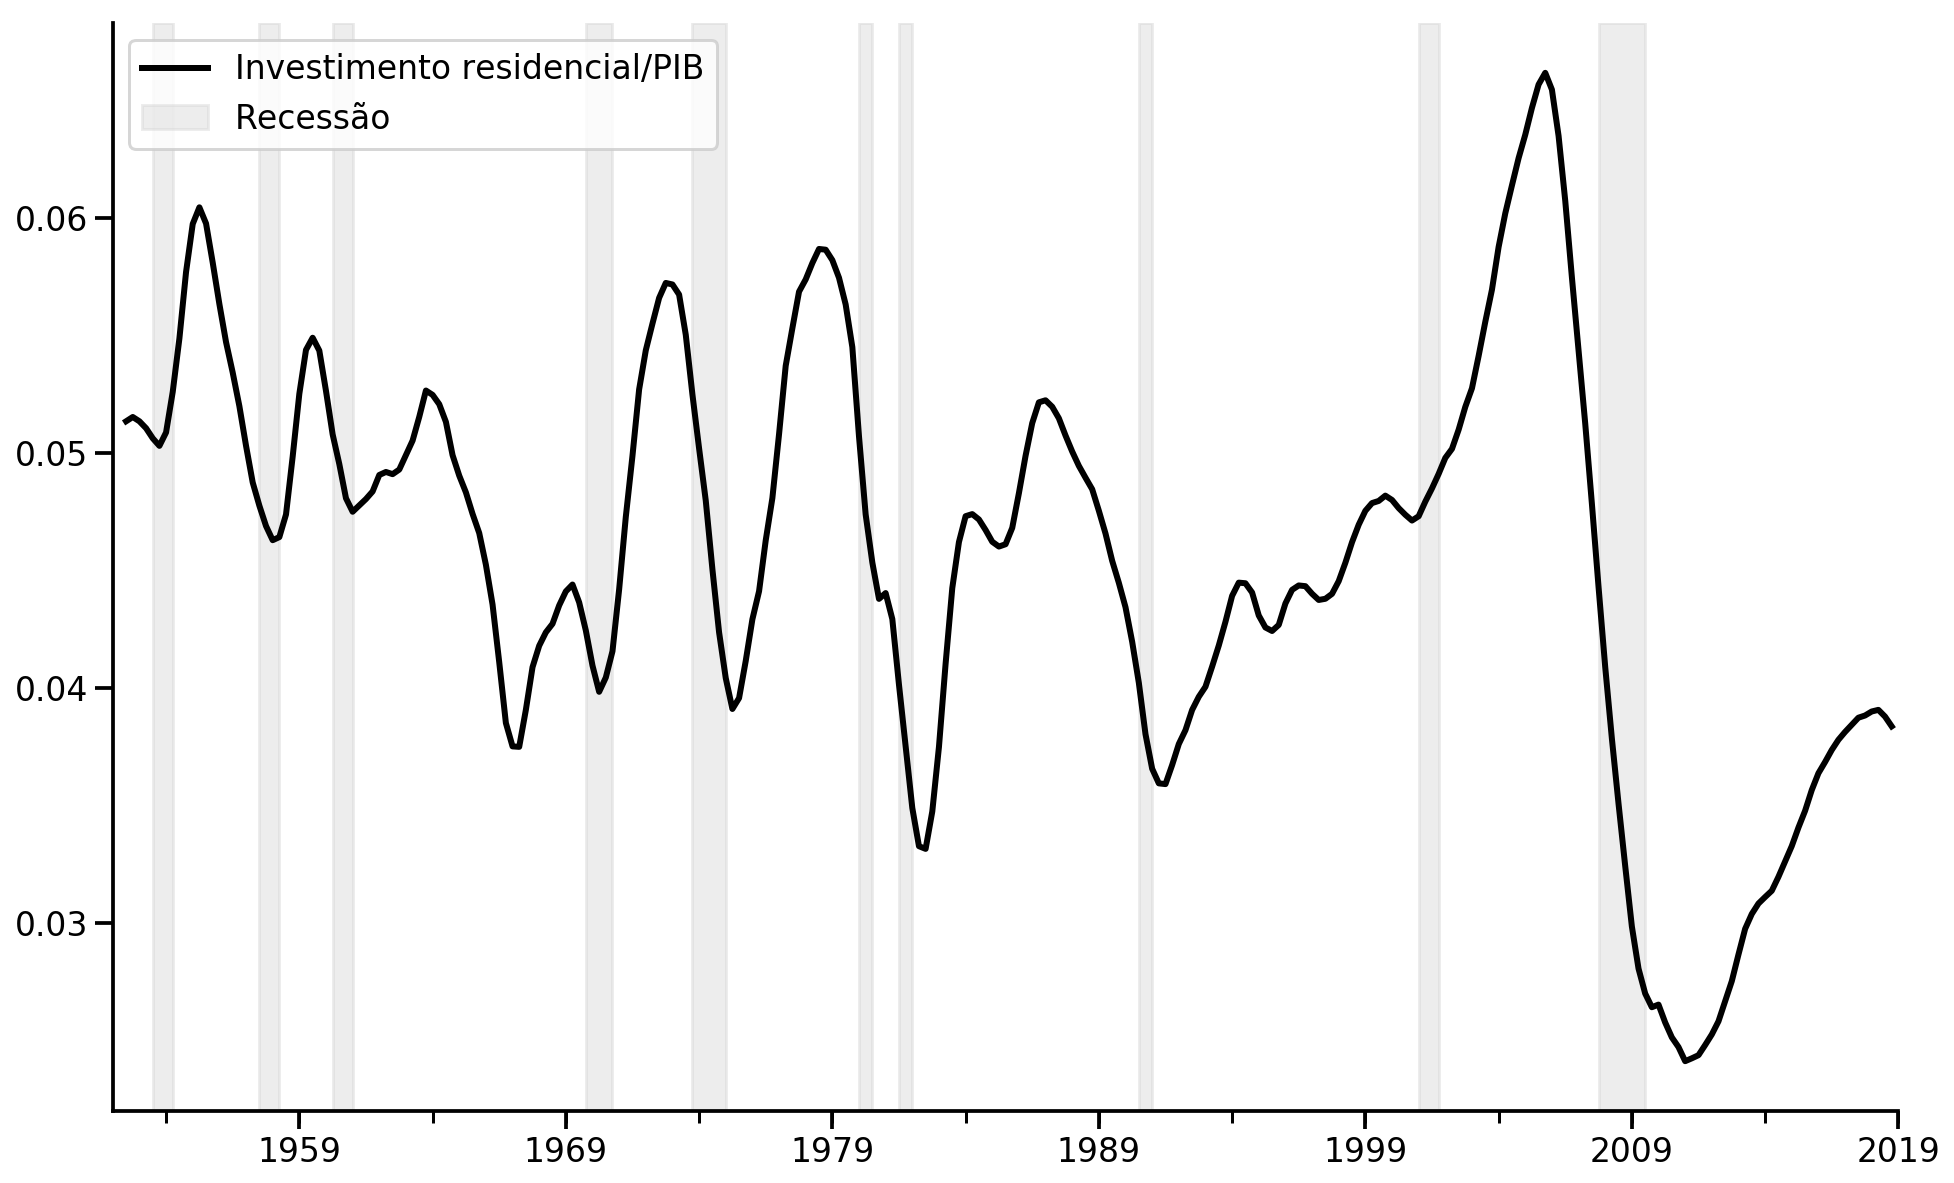
\includegraphics[width = 0.7\textwidth]{Introducao/InvtResiden_PIB.png}
    \label{Investo_Resid_GDP}
    \caption*{\textbf{Fonte:} Federal Reserve Bank of St. Louis, elaboração dos autores.}
\end{figure} 

O gráfico \ref{Investo_Resid_GDP} mostra como a compreensão da dinâmica do investimento residencial pode antecipar recessões. No período apresentado (1952Q1-2018Q4), verifica-se que as recessões são antecedidas por uma redução na taxa de investimento residencial enquanto a retomada pode ser caracterizada por uma ampliação deste gasto. Vale pontuar que a recessão de 1966-67 foge deste comportamento por conta do aumento dos gastos do governo associado a guerra do Vietnã e, portanto, configurando um falso positivo \cite[p.~20]{leamer_housing_2007}. Outra exceção é a crise das bolhas-ponto-com que não apresentou relação direta com o investimento residencial. Já a crise do \textit{subprime}, por sua vez, é a que apresenta esse comportamento de forma mais acentuada. Portanto, o investimento das famílias é relevante para o entendimento da dinâmica da economia norte-americana.

\begin{figure}[htb]
    \centering
        \caption{Taxa de investimento residencial e grau de utilização ao longo dos ciclos} 
        \caption*{(Tamanho dos pontos indica os anos)}
    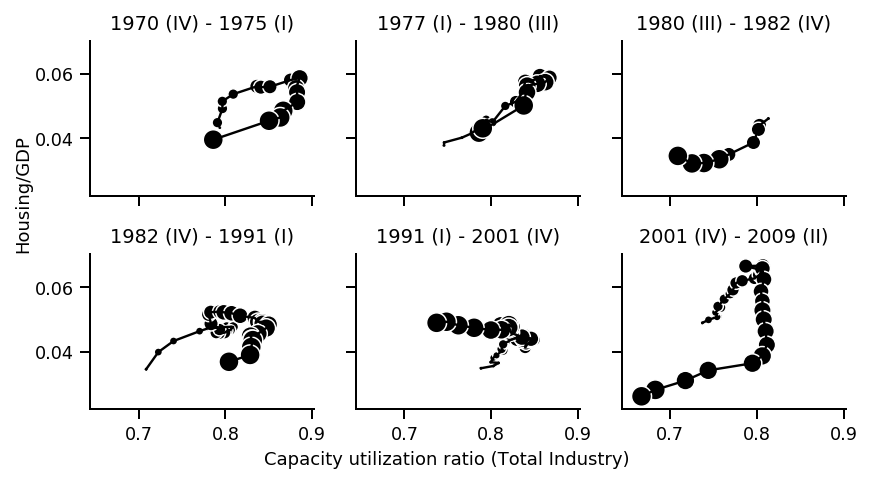
\includegraphics[width = 0.65\textwidth]{Introducao/Empiria_AKB.png}
    \label{Investo_Resid}
    \caption*{\textbf{Fonte:} Federal Reserve Bank of St. Louis, elaboração dos autores.}
\end{figure}

Outra forma de compreender a importância do investimento residencial para o ciclo econômico nos EUA pode ser vista no gráfico \ref{Investo_Resid} a seguir em que cada um dos painéis apresenta um ciclo\footnote{Raciocínio semelhante pode ser encontrado em \textcite{fiebiger_semi-autonomous_2018}.}. No eixo vertical, vemos a participação desse gasto no PIB, enquanto no eixo horizontal, temos o grau de utilização da capacidade como uma \textit{proxy} para o ciclo econômico. Exceto para o período 1991-2001, a recuperação (aumento da utilização da capacidade) é caracterizada por uma taxa de crescimento do investimento residencial maior que o crescimento da economia, resultando em maior participação desse gasto no PIB. Considerando que as firmas seguem o princípio do ajuste do estoque de capital, ampliam a taxa de acumulação de modo a ajustar o grau de utilização para o grau normal. O aumento da taxa de crescimento do investimento das firmas e de outros gastos reduz a participação do investimento residencial no PIB. A maturação do investimento das firmas, por sua vez, redunda em menor utilização da capacidade produtiva\footnote{Complementarmente, os trabalhos de \textcite{fiebiger_semi-autonomous_2018} e \textcite{fiebiger_trend_2017} também reportam o investimento residencial como determinante do comportamento cíclico e adicionam o consumo financiado por crédito a essa dinâmica. Além disso, apresentam uma similaridade com \textcite{dejuan_hidden_2017} e \textcite{teixeira_crescimento_2015} para os quais a instabilidade econômica está associada à instabilidade (ao menos de alguns) gastos autônomos e não do investimento das firmas, que segue o princípio do ajuste do estoque de capital.}. Desse modo, conclui-se que o investimento residencial ajuda a compreender grande parte das recessões desde o pós-guerra.

Compreendida a importância do investimento residencial para a dinâmica econômica, caberá ao segundo capítulo analisar alguns fatos estilizados da economia norte-americana da década de 80 em diante. A justificativa deste recorte temporal se dá tanto pela estagnação dos salários e subsequente piora na distribuição pessoal da renda \cites{barba_rising_2009}{teixeira_uma_2011} quanto pela maior representatividade das hipotecas nos balanços patrimoniais dos bancos \cite{jorda_great_2014}. Adicionalmente, pretende-se estimar um modelo de séries temporais e, portanto, avalia-se a pertinência de um VAR/VECM ou ARDL de modo a captar de forma mais adequada os determinantes do investimento residencial e testar a hipótese de que  a taxa própria de juros dos imóveis, como definida em \textcite{teixeira_crescimento_2015}, contribui para compreender o caso norte-americano.

%CAPÍTULO MODELO

Diante dos fatos estilizados destacados, constrói-se, no capítulo seguinte, um modelo SFC de modo a incluir o investimento residencial. A razões por se optar por esta metodologia decorre da capacidade de tratar de maneira satisfatória das relações financeiras entre os diferentes setores institucionais. Na presente versão da pesquisa, é apresentado um modelo em sua forma mais simplificada de modo a captar a dinâmica entre dois tipos de estoque de capital: das firmas (criador de capacidade) e das famílias. Até o momento, são identificadas algumas limitações (ver apêndice \ref{Append_Fraction}) que devem ser contornadas em outras versões. Futuramente, pretende-se incluir uma dinâmica de preços de modo que seja possível captar a importância da inflação de ativos e de ganhos de capital. 

%Conclusões

Portanto, a presente investigação estende as contribuições de \textcite{serrano_sraffian_1995} ao incluir o investimento residencial na agenda de pesquisa do supermultiplicador sraffiano, de \textcite{teixeira_crescimento_2015} ao incorporar o conceito de taxa próprio de juros dos imóveis para avaliar a dinâmica de tal gasto autônomo e a de \textcite{brochier_supermultiplier_2018} por adicionar um tratamento adequado das relações financeiras no SSM por meio da metodologia SFC.

\end{comment}